\begin{enumerate}[label=\thechapter.\arabic*,ref=\thechapter.\theenumi]

\item The damping ratio and undamped natural frequency of a closed loop system as
shown in the figure, are denoted as $\zeta$ and $\omega_n$, respectively. The values of $\zeta$ and $\omega_n$
are 
\begin{figure}[!ht]
\centering
\begin{center}
\includegraphics[width=\columnwidth]{2022/EE/39/figs/question.jpg}
\end{center}
%\caption{Diagram for GATE ME Question 30}
\end{figure}
\begin{enumerate}
    \item $\zeta = 0.5$ and $\omega_n = 10$ rad/s
    \item $\zeta = 0.1$ and $\omega_n = 10$ rad/s
    \item $\zeta = 0.707$ and $\omega_n = 10$ rad/s
    \item $\zeta = 0.707$ and $\omega_n = 100$ rad/s
\end{enumerate}
\hfill(GATE EE 2022)
\solution
\iffalse
\let\negmedspace\undefined
\let\negthickspace\undefined
\documentclass[journal,12pt,twocolumn]{IEEEtran}
\usepackage{cite}
\usepackage{amsmath,amssymb,amsfonts,amsthm}
\usepackage{algorithmic}
\usepackage{graphicx}
\usepackage{textcomp}
\usepackage{xcolor}
\usepackage{txfonts}
\usepackage{listings}
\usepackage{enumitem}
\usepackage{mathtools}
\usepackage{gensymb}
\usepackage{comment}
\usepackage[breaklinks=true]{hyperref}
\usepackage{tkz-euclide} 
\usepackage{listings}
\usepackage{gvv}                                        
\def\inputGnumericTable{}                                 
\usepackage[latin1]{inputenc}                                
\usepackage{color}                                            
\usepackage{array}                                            
\usepackage{longtable}                                       
\usepackage{calc}                                             
\usepackage{multirow}                                         
\usepackage{hhline}                                           
\usepackage{ifthen}                                           
\usepackage{lscape}
\usepackage{placeins}
\usepackage{xparse}


\newtheorem{theorem}{Theorem}[section]
\newtheorem{problem}{Problem}
\newtheorem{proposition}{Proposition}[section]
\newtheorem{lemma}{Lemma}[section]
\newtheorem{corollary}[theorem]{Corollary}
\newtheorem{example}{Example}[section]
\newtheorem{definition}[problem]{Definition}
\newcommand{\BEQA}{\begin{eqnarray}}
\newcommand{\EEQA}{\end{eqnarray}}
\newcommand{\define}{\stackrel{\triangle}{=}}
\theoremstyle{remark}
\newtheorem{rem}{Remark}

\graphicspath{ {./figs/} } 

\begin{document}

\bibliographystyle{IEEEtran}
\vspace{3cm}

\Large\title{GATE 2022 EE 39}
\large\author{EE23BTECH11032 - Kaustubh Parag Khachane $^{*}$% <-this % stops a space
}
\maketitle
\newpage
\bigskip

\renewcommand{\thefigure}{\theenumi}
\renewcommand{\thetable}{\theenumi}
\large\textbf{Question GATE 22 EE 39} :\\
The damping ratio and undamped natural frequency of a closed loop system as
shown in the figure, are denoted as $\zeta$ and $\omega_n$, respectively. The values of $\zeta$ and $\omega_n$
are 
\begin{figure}[!ht]
\centering
\begin{center}
\includegraphics[width=\columnwidth]{question}
\end{center}
%\caption{Diagram for GATE ME Question 30}
\end{figure}
\begin{enumerate}
    \item $\zeta = 0.5$ and $\omega_n = 10$ rad/s
    \item $\zeta = 0.1$ and $\omega_n = 10$ rad/s
    \item $\zeta = 0.707$ and $\omega_n = 10$ rad/s
    \item $\zeta = 0.707$ and $\omega_n = 100$ rad/s
\end{enumerate}
\hfill(GATE EE 2022)\\
\solution\\
\fi
\begin{table}[!ht] 
\centering
\setlength{\extrarowheight}{8pt}
\begin{tabular}{|l|l|l|}
    \hline
    \textbf{Parameter} & \textbf{Description} & \textbf{Values}\\
    \hline
     m & load of system &  \\
    \hline
     k & stiffness of system &  \\
    \hline
     $\omega_n$ & Natural frequency & $\sqrt{\frac{k}{m}}$ \\
    \hline
    $\zeta$ & Damping ratio & $\frac{c}{2m\omega_n}$ \\
    \hline
     y\brak{t} & Output of system & \\
    \hline
     x\brak{t} & Input to the system & \\
    \hline
     c & Damping coefficient & \\
    \hline
    T\brak{s} & Transfer function of system & $\frac{Y\brak{s}}{R\brak{s}}$\\
    \hline
  \end{tabular}
  \vspace{4mm}
 \caption{Parameter Table}
 \label{tab:table0_ee_22_39}
\end{table}

We will use Mason's Gain Formula to calculate the transfer function of this system. First converting the given diagram to a signal flow graph :

\begin{figure}[!ht]
\centering
\resizebox{0.5\textwidth}{!}{%
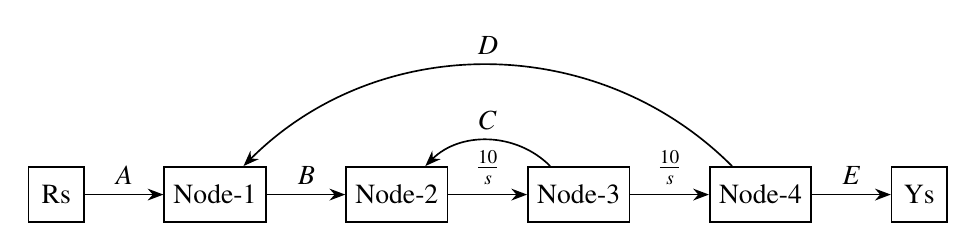
\begin{tikzpicture}[>=Stealth,auto,node distance=1cm,semithick]
  \tikzstyle{block}=[draw, fill=white, rectangle, minimum height=2em, minimum width=2em]
  
  \node [block] (input) {R\brak{s}};
  \node [block, right=of input] (filter) {Node-1};
  \node [block, right=of filter] (D) {Node-2};
  \node [block, right=of D] (E) {Node-3};
  \node [block, right=of E] (F) {Node-4};
  \node [block, right=of F] (output) {Y\brak{s}};
  
  \draw [->] (input) -- node {$A$} (filter);
  \draw [->] (filter) -- node {$B$} (D);
  \draw [->] (D) -- node {$\frac{10}{s}$} (E);
  \draw [->] (E) -- node {$\frac{10}{s}$} (F);
  \draw [->] (F) -- node {$E$} (output);
  
  % Backward loops
  \draw [->] (E) edge [bend right=45] node[above] {$C$} (D);
  \draw [->] (F) edge [bend right=45] node[above] {$D$} (filter);
\end{tikzpicture}%
}
\caption{Signal Flow Diagram}
\label{fig:your_label}
\end{figure}


Mason's Gain Formula is given by :
\begin{align}
    H\brak{s} = \sum_{i=1}^{N}\brak{\frac{P_i \Delta_i}{\Delta}} \label{eq:eq1_ee39}
\end{align}
\begin{table}[!ht] 
\centering
\setlength{\extrarowheight}{8pt}
\begin{tabular}{|l|l|}
    \hline
    \textbf{Parameter} & \textbf{Description}\\
    \hline
     N & Number of forward paths \\\hline
     L & Number of loops\\\hline
     $P_k$ & Forward path gain of $k^{th}$ path\\\hline
     $\Delta_k$ & Associated path factor \\\hline
     $\Delta$ & Determinant of the graph \\\hline
  \end{tabular}
  \vspace{4mm}
 \caption{Parameter Table - Mason's Gain Law}
 \label{tab:table1_ee_22_39}
\end{table}

\begin{table}[!ht] 
\centering
\setlength{\extrarowheight}{8pt}
\begin{tabular}{|l|l|}
    \hline
    \textbf{Parameter} & \textbf{Formula}\\
    \hline
     $\Delta$ & 1 + $\sum_{k=1}^{L}\brak{\brak{-1}^k\text{Product of gain of groups of k isolated loops}}$ \\\hline
     $\Delta_k$ & $\Delta$ part of graph that is not touching $k^{th}$ forward path \\\hline
  \end{tabular}
  \vspace{4mm}
 \caption{Formula Table - Mason's Gain Law}
 \label{tab:table2_ee_22_39}
\end{table}

This signal flow graph has only one forward path whose gain is given by :
\begin{align}
    P_1 &= \frac{10}{s} \frac{10}{s}\\
    &= \frac{100}{s^2}
\end{align}
The loop gain for loop between Node-2 and Node-3 is :
\begin{align}
    L_1 &= \frac{10}{s}\brak{-1}\\
    &= -\frac{10}{s}
\end{align}
The loop gain for loop between Node-1 and Node-4 is :
\begin{align}
    L_1 &= \frac{10}{s}\frac{10}{s}\brak{-1}\\
    &= -\frac{100}{s^2}
\end{align}
Using \tabref{tab:table2_ee_22_39}, $\Delta$ is :
\begin{align}
    \Delta &= 1 - \brak{-\frac{10}{s} - \frac{100}{s^2}}\\
    &= 1 + \frac{10}{s} + \frac{100}{s^2}
\end{align}
There are no two isolated loops available. Hence all further terms will b zero.\\
As both the loops are in contact with the only forward path,
\begin{align}
    \Delta_1 = 1
\end{align}
Using equation \eqref{eq:eq1_ee39} :
\begin{align}
    H\brak{s} &= \frac{\frac{100}{s^2}}{1 + \frac{10}{s} + \frac{100}{s^2}} \\
    &= \frac{100}{s^2 + 10s + 100}\label{eq:eq2_ee39}
\end{align}
Referring to \tabref{tab:table0_ee_22_39}, the general equation of the damping system is second order and can be written as :
\begin{align}
    m\ddot{y}(t) + c\dot{y}(t) + ky(t) = x(t)
\end{align}
Take the Laplace transform and solve for $\frac{Y\brak{s}}{X\brak{s}}$ :
\begin{align}
    \frac{Y\brak{s}}{X\brak{s}} &= \frac{\omega_n^2}{s^2 + 2\zeta\omega_n s + \omega_n^2}\\
\implies H\brak{s} &= \frac{\omega_n^2}{s^2 + 2\zeta\omega_n s + \omega_n^2} \label{eq:eq3_ee39}
\end{align}
Comparing equations \eqref{eq:eq2_ee39} and \eqref{eq:eq3_ee39} ,
\begin{align}
    \omega_n ^2 &= 100\\
    \implies \omega_n &= 10 \text{ rad/s} \label{eq:eq4_ee39}\\
    2\zeta \omega_n &= 10\\
    \implies \zeta &= 0.5
\end{align}
\begin{figure}[!ht]
\centering
\begin{center}
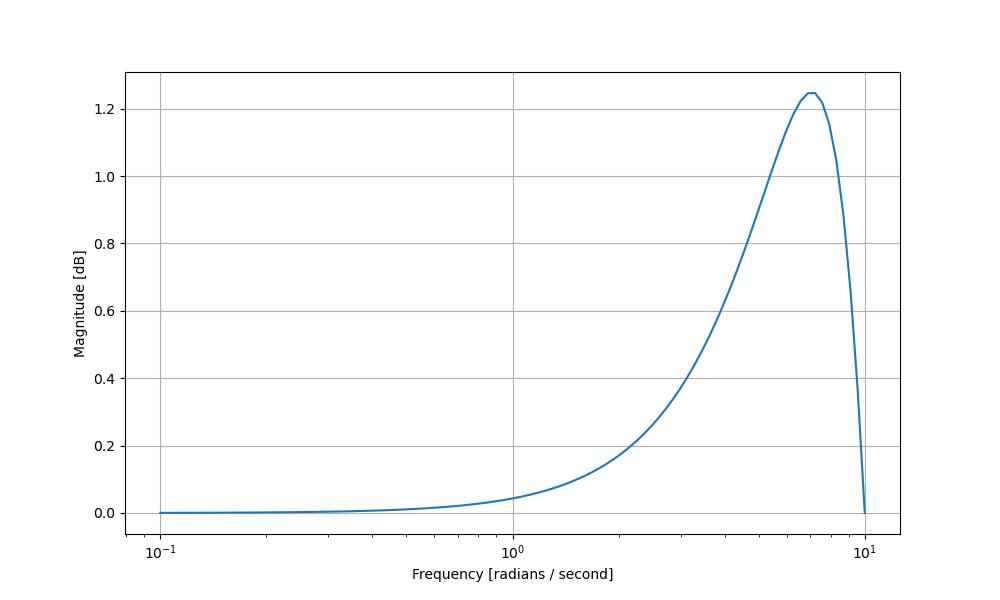
\includegraphics[width=\columnwidth]{2022/EE/39/figs/Figure_1.jpg}
\end{center}
\caption{Magnitude plot}
\end{figure}
\begin{figure}[!ht]
\centering
\begin{center}
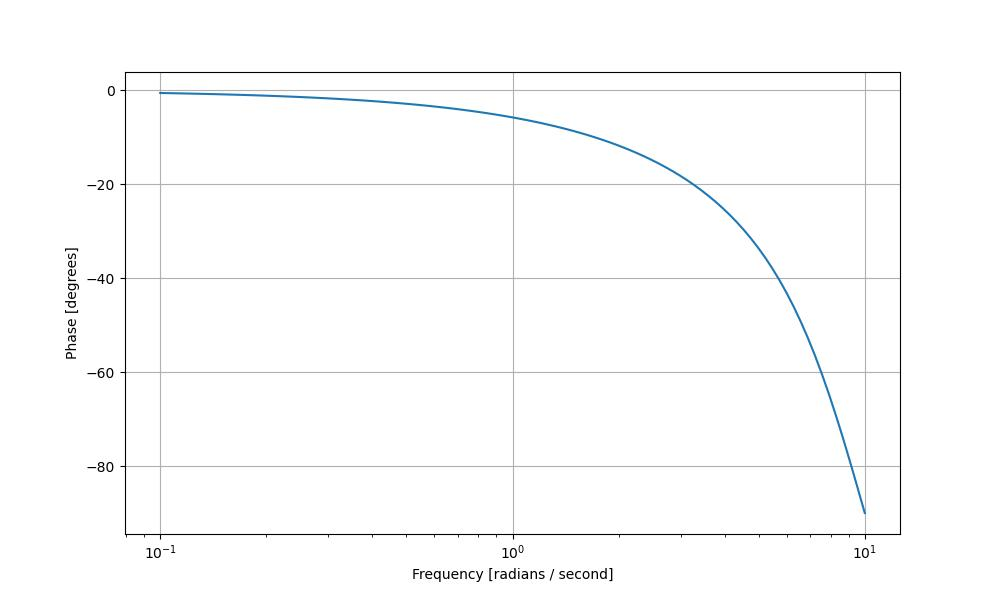
\includegraphics[width=\columnwidth]{2022/EE/39/figs/Figure_2.jpg}
\end{center}
\caption{Phase plot}
\end{figure}

\newpage
\item In the block diagram shown in the figure, the transfer function $G=\frac{K}{\tau s+1}$ with $K>0$ and $\tau>0$. The maximum value of $K$ below which the system remains stable is \rule{1cm}{0.15mm}(rounded off to two decimal places) \hfill (GATE CH 2022) 
\begin{figure}[htbp] 
\includegraphics[width=\columnwidth]{2022/CH/58/figs/question.jpg} 
\end{figure}\\ 
\solution 
\input{2022/CH/58/ch_58.tex} 
\newpage

\item
A series RLC circuit is connected to 220 V, 50 Hz supply. For a fixed a value of R and C, the inductor L is varied to deliver the maximum current. This value 0.4A and the corresponding potential drop across the capacitor is 330 V. The value of the inductor L is ? (Rounded off to two decimal places).
\hfill{(GATE BM 2022)}\\
 \solution
 \iffalse
\let\negmedspace\undefined
\let\negthickspace\undefined
\documentclass[journal,12pt,onecolumn]{IEEEtran}
\usepackage{cite}
\usepackage{amsmath,amssymb,amsfonts,amsthm}
\usepackage{algorithmic}
\usepackage{graphicx}
\usepackage{textcomp}
\usepackage{xcolor}
\usepackage{txfonts}
\usepackage{listings}
\usepackage{enumitem}
\usepackage{circuitikz}
\usepackage{mathtools}
\usepackage{gensymb}
\usepackage{comment}
\usepackage[breaklinks=true]{hyperref}
\usepackage{tkz-euclide} 
\usepackage{listings}
\usepackage{gvv}    
\usepackage{enumitem}
\usepackage{amsmath}
\def\inputGnumericTable{}                                 
\usepackage[latin1]{inputenc}                                
\usepackage{color}                                            
\usepackage{array}                                            
\usepackage{longtable}                                       
\usepackage{calc}                                             
\usepackage{multirow}                                         
\usepackage{hhline}                                           
\usepackage{ifthen}                                           
\usepackage{lscape}
\usepackage{tabularx}

\newtheorem{theorem}{Theorem}[section]
\newtheorem{problem}{Problem}
\newtheorem{proposition}{Proposition}[section]
\newtheorem{lemma}{Lemma}[section]
\newtheorem{corollary}[theorem]{Corollary}
\newtheorem{example}{Example}[section]
\newtheorem{definition}[problem]{Definition}
\newcommand{\BEQA}{\begin{eqnarray}}
\newcommand{\EEQA}{\end{eqnarray}}
\newcommand{\define}{\stackrel{\triangle}{=}}
\theoremstyle{remark}
\newtheorem{rem}{Remark}
\begin{document}
\bibliographystyle{IEEEtran}
\vspace{3cm}

\title{GATE:2022 - BM 54 }
\author{EE23BTECH11025 - Anantha Krishnan $^{}$% <-this % stops a space
}
\maketitle
\bigskip



\section{question}

A series RLC circuit is connected to 220 V, 50 Hz supply. For a fixed a value of R and C, the inductor L is varied to deliver the maximum current. This value 0.4A and the corresponding potential drop across the capacitor is 330 V. The value of the inductor L is ? (Rounded off to two decimal places).
 



\textbf{Solutions :}
\fi




\begin{table}[ht!]
\centering
\begin{tabular}{ |c|c|c| } 
 \hline
Symbols & Description & Values  \\
\hline
 $V_s$ & Input voltage & 220 V and 50Hz\\
 \hline
 $\chi_L$ & Impedance across inductor & $j\omega L$\\
 \hline
 $\chi_C$ & Impedance across capacitor & $\frac{-j}{\omega C}$\\
 \hline
 $Z$& Impedance across the entire circuit & $\frac{1}{R+j\omega L +\frac{-j}{\omega C}}$\\
 \hline
\end{tabular}
\caption{Parameters, Descriptions, and Values}
\label{table:ee25-bm54-gate2022}
\end{table}






    
    \ctikzset{bipoles/thickness=1.2}
    \newcommand{\midlabelline}[3]{
   \node (midlabel) at ($ (#1)!.5!(#2) $) {#3};
   \draw[latex-] (#1) --  (midlabel);
   \draw[-latex] (midlabel) -- (#2);
}

\begin{enumerate}
\begin{center}
\begin{circuitikz}[scale=0.8]
    % Circuit
    \draw[line width=0.6]
        (1.5,5) to [sinusoidal voltage source, l_=$220V$${,}50Hz$, i=$I$] (1.5,1)
        (1.5,5) to [resistor, l_=$R$] ++(4,0) to [inductor, l_=$L$] ++(0,-4) to [capacitor, l_=$C$] +(-4,0) ;
    
    % Voltage Infos
    \midlabelline{1.5,5.5}{5.5,5.5}{$V(R)$}
    \midlabelline{6.5,5}{6.5,1}{$V(L)$}
    \midlabelline{1.5,0}{5.5,0}{$V(C)$}
    
    % Grid
    %\draw[help lines] (0,0) grid (7,6);
\end{circuitikz}
\end{center}
    \end{enumerate}
During maximum current$\quad\abs{Z}$ is minimum .
\begin{align}
I &= \frac{V_s}{Z}\\
 &= \frac{V_s}{R+\chi_{L}+\chi_{C}}\\ 
 &=\frac{V_s}{R+j\omega L+\frac{1}{j\omega C}}\label{eq:ee25-gate2-1}\\
\quad \abs{I}&={\frac{\quad \abs{V_s}}{\sqrt{R+\brak{\omega L-\frac{1}{\omega C}^2}}}}
\end{align}
Varying $L$ for maximum value of ${I}$ :
\begin{align}
\omega L = \frac{1}{\omega C} \label{eq:ee25-gate2-2}
\end{align}
Putting in $\eqref{eq:ee25-gate2-1}$:
\begin{align}
    I_{max} &= \frac{V_s}{R}
\end{align}
$I_{max}$ has same phase as $V_s$ (Assume $\angle{\phi})$.
For impedance across the capacitor :
\begin{align}
 \left.V_C\right|_{I=I_{max}}&= I_{max} \chi_C\\
-330\angle{\brak{90+\phi}} &= \brak{0.4\angle{\phi}}\chi_C\\
-330\angle{90} &= 0.4\chi_C\\
\implies \chi_C &= -825j\si{\ohm}
\end{align}
For value of Capacitor and inductor, using \eqref{eq:ee25-gate2-2} :
\begin{align}
L &= \frac{825}{100\pi}H\\
&\approx 2.63 \si{H}\\
C &= 3.858*10^{-6} \si{F}
\end{align}


    \begin{figure}[!ht]    
    \centering
\graphicspath{ {2022/BM/54/figs/} }
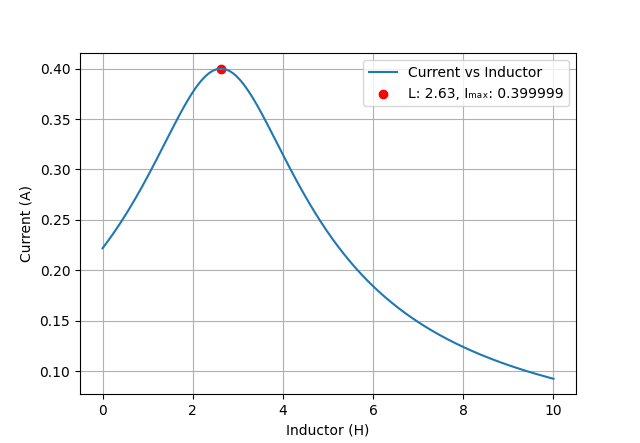
\includegraphics[width=\columnwidth]{graph_1}
\caption{ $I$ vs $L$ }
\label{graph:ee25-gate2-graph}
\end{figure}







 
 \newpage
 
 \item
 The open loop transfer function of a unity gain negative feedback system is given by $G\brak{s}= \frac{k}{s^2 +4s-5}$. The range of k for which the system is stable,is\hfill(GATE EE 2022)\\
\solution
\iffalse
\documentclass[journal,12pt,twocolumn]{IEEEtran}
\usepackage{amsmath,amssymb,amsfonts,amsthm}
\usepackage{txfonts}
\usepackage{tkz-euclide}
\usepackage{listings}
\usepackage{gvv}
\usepackage[latin1]{inputenc}
\usepackage{array}
\usepackage{pgf}
\usepackage{lmodern}
\usepackage{amsmath}
\begin{document}
\bibliographystyle{IEEEtran}

\title{GATE 2022[EE]-19}
\author{EE23BTECH11066 - Yakkala Amarnath Karthik}
\maketitle
\bibliographystyle{IEEEtran}

\textbf{Question:}\\ \\
The open loop transfer function of a unity gain negative feedback system is given by $G\brak{s}= \frac{k}{s^2 +4s-5}$. The range of k for which the system is stable,is\hfill(GATE EE 2022)\\ \\

\textbf{Solution:}\\ 
\fi
\begin{table}[ht]
  \begin{tabular}{|c|c|c|}
    \hline
    \textbf{Variable} & \textbf{Description} & \textbf{value}\\
    \hline
    $G\brak{s}$ & Open loop transfer function & $\frac{k}{s^2 +4s-5}$\\
   \hline
    1+G$\brak{s}$ & Characteristic equation & 0 \\
    \hline
    \end{tabular}
  \caption{A Table with input parameters}
  \label{tab:gate2022ee19}
\end{table}
\\
 from Table\ref{tab:gate2022ee19}\\
Characteristic equation:
\begin{align}
    1+G\brak{s}=0\\
    \implies 1+\frac{k}{s^2 +4s-5}=0\\
    \implies s^2+4s+\brak{k-5}=0
\end{align}
By routh table analysis, for a stable system:

\begin{center}
    \begin{tabular}{c|c c}
        $s^2$ & 1 & \(k-5\) \\
        $s^1$ & 4 & 0 \\
        $s^0$ & \(\frac{4\brak{k-5}-0}{4}\) & 0 \\
    \end{tabular}
\end{center}


\begin{align}
\frac{4\brak{k-5}-0}{4}>0\\
    k-5>0\\
    \implies k>5
\end{align}

\begin{figure}[ht]
    \centering
    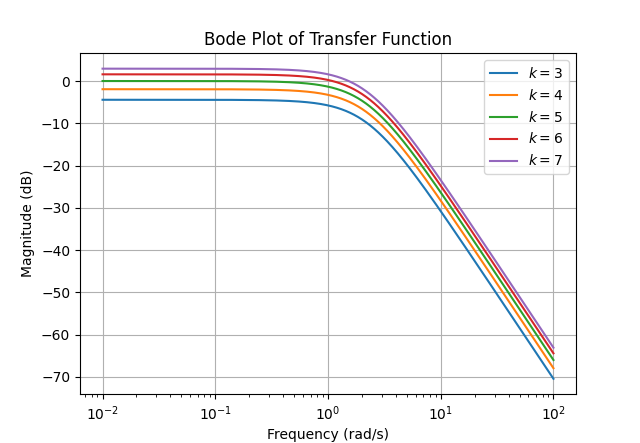
\includegraphics[width=0.45\textwidth]{2022/EE/19/figs/bodeplot.png}
    \caption{Graph showing $k<5,k=5,k>5$}
\end{figure}
For an open transfer function to be stable, its magnitude in the bode plot should be positive for some positive frequency.\\
In the below graph we can observe that the above condition satisfies for k$>$5. 
%\end{document}

\newpage

\item
The block diagrams of an ideal system and a real system with their impulse
responses are shown below. An auxiliary path is added to the delayed impulse
response in the real system.\\
\\
For a unit impulse input $\brak{x\brak{t}} = \delta \brak{t}${ to both systems, gain $\beta$ is chosen such that $y \brak{4T}$ is same for both systems. The value of $\beta$ is:
\begin{figure}[ht]
    \centering
    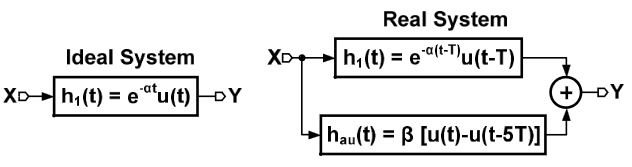
\includegraphics[width=\columnwidth]{2022/BM/40/figs/fig3.png}
    \label{fig: 10.5.3.128}
\end{figure}
\\
$\brak{A} e^{-3 \alpha T} \brak{1 - e^{-2 \alpha T}}$\\
\\
$\brak{B} -e^{- \alpha T} \brak{1 - e^{-3 \alpha T}}$\\
\\
$\brak{C} -e^{-3 \alpha T} \brak{1 - e^{-\alpha T}}$\\
\\
$\brak{D} e^{-2 \alpha T} \brak{1 - e^{-2 \alpha T}}$\\
\hfill{(GATE BM 2022)}\\
 
\end{enumerate}
